\section{Implementation}


\begin{figure}[ht]
    \centering
    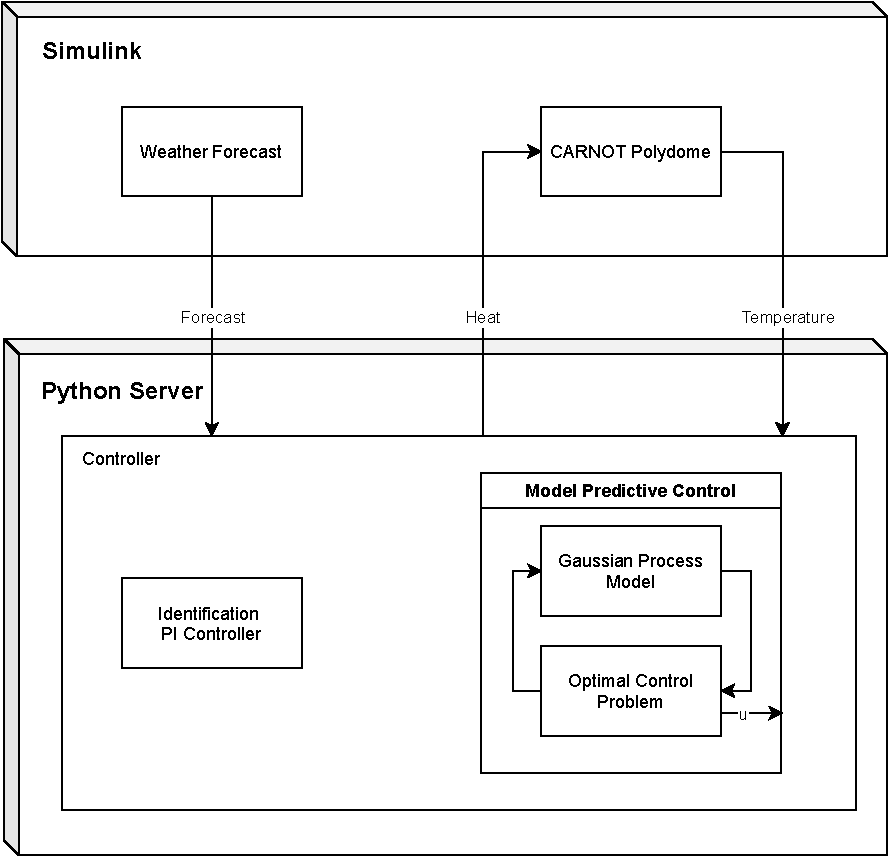
\includegraphics[width = 0.5\textwidth]{Images/setup_diagram.pdf}
    \caption{Block diagram of the Simulink plant and Python Controller}
    \label{fig:setup_diagram}
\end{figure}


% TODO: [Implementation] Reference implementation details for CARNOT and WDB

\subsection{Gaussian Processes}

% TODO: [Implementation] Cite Tensorflow
% TODO: [Implementation] Cite GPflow

\subsection{Classical Gaussian Process training}
\subsection{Sparse and Variational Gaussian Process training}


\subsection{Optimal Control Problem}
\subsubsection{Sparse Implementation of the Optimization Problem}

The optimization problem as presented in
Equation~\ref{eq:optimal_control_problem} becomes very nonlinear quite fast. In
fact, due to the autoregressive structure of the \acrshort{gp}, the predicted
temperature at time t is passed as an input to the model at time $t+1$. A simple
recursive implementation of the Optimization Problem becomes untractable after
only 3 --- 4 prediction steps. 

In order to solve this problem, a new OCP is introduced. It has a much sparser
structure, in exchange for a larger number of variables. This turns out to be
much faster to solve than the original problem.

Let $w_l$, $u_l$, and $y_l$ be the lengths of the state vector components
$\mathbf{w}$, $\mathbf{u}$, $\mathbf{y}$ (cf. Equation~\ref{eq:components}).

\begin{subequations}\label{eq:sparse_optimal_control_problem}
    \begin{align}
        & \text{minimize}
        & & \sum_{i=2}^{N + 1} \left(X[i, w_l + u_l + 1] - y_{ref, t}\right)^2 \\
        & \text{subject to}
        & & X[i+1, w_l + u_l + 1] = K_*K^{-1}X[i, :] \quad \text{for} \quad
        i\in[1, N]\\
        &&& X[i, w_l + u_l + 2: ] = X[i, w_l+ u_l + 1: w_l + u_l + y_l - 1]\\
        &&& X[i, 1:w_l] = W[i, :] \\
        &&& X[i+1, w_l + 2: w_l + u_l] = X[i, w_l + 1: w_l + u_l - 1] \\
        &&& X[:, w_l + 1] \in \mathcal{U}
    \end{align}
\end{subequations}

where X is the matrix of all the system states and W is the matrix of the
disturbances.

\subsubsection{RENAME: Python implementation of the control problem}
% TODO: [Implementation] Cite CasADi
% TODO: [Implementation] Cite HSL solvers for using MA27


\subsection{Python server and controller objects}


\clearpage
